\documentclass[letterpaper]{article}
\usepackage{aaai2027}
\usepackage[hyphens]{url}
\usepackage{graphicx}
\urlstyle{rm}
\def\UrlFont{\rm}
\usepackage{natbib}
\usepackage{caption}
\frenchspacing
\usepackage{booktabs}
\usepackage{amsmath}
\usepackage{xcolor}
\usepackage{tikz}
\usetikzlibrary{positioning}
\pdfinfo{
/TemplateVersion (2027.2)
}
\setcounter{secnumdepth}{2}
\nocopyright  % course report, not an AAAI publication
\newcommand{\todo}[1]{\colorbox{yellow}{#1}}

\title{A Distilled 4.8M-Parameter ResNet for CIFAR-10}
\author{
    Mirsaid Abbasov (ma9197), solo team
}
\affiliations{
    NYU Tandon School of Engineering, Deep Learning (Fall 2026), Project 1\\
    Code: \url{https://github.com/ma9197/dl-project1-resnet}\\
    Kaggle team: Abbasov
}

\begin{document}

\maketitle

\begin{abstract}
I designed and trained, from scratch, a residual network for CIFAR-10 with at most 5 million trainable parameters.
The final model has three residual layers with 84, 168 and 336 channels and two basic blocks per layer
(4,781,374 parameters). The recipe has three parts: a layout that spends the parameter budget on width at high
resolution, strong data augmentation (crop, flip, Cutout, TrivialAugment and CutMix) with a long cosine schedule, and
knowledge distillation from larger teachers that are used only during training. The plain model reaches 96.73\%
on the CIFAR-10 test set (97.00\% when averaging an image and its mirror image); the distilled model with the same
architecture reaches 97.82\% (97.89\%). On the competition's held-out test set it scores 0.907 on the public
leaderboard, up from 0.884 for the plain model, and my final entry scores 0.874 on the hidden half (rank 28 of 81). Main findings: (1) three wide residual layers beat ResNet-18 style
four-layer layouts at this budget; (2) the training recipe mattered more than the layout; (3) distillation with long
training added about 0.9 points on CIFAR-10 at no inference cost; (4) on the competition images, which come from a
shifted distribution, more CutMix raised the score more than its CIFAR-10 accuracy suggested; (5) test-time
adjustments that looked harmless on CIFAR-10 lowered the competition score, so I did not use them.
\end{abstract}

\section{Introduction}
A residual network (ResNet) \cite{he2016deep} is a convolutional network built from residual blocks that compute
$\mathrm{ReLU}(S(x) + F(x))$, where $F$ is conv $\rightarrow$ BN $\rightarrow$ ReLU $\rightarrow$ conv
$\rightarrow$ BN \cite{ioffe2015batch} and $S$ is the skip connection. The task is to find the most accurate
modified ResNet on a held-out version of CIFAR-10 \cite{krizhevsky2009learning} (2,000 images with hidden labels,
scored by accuracy on Kaggle), with two rules: at most 5,000,000 trainable parameters, and no pretrained weights or
extra data. The design variables are the number of residual layers $N$, and for layer $i$ the number of blocks
$B_i$, channels $C_i$, conv kernel size $F_i$ and skip kernel size $K_i$, plus the average-pool size $P$.
ResNet-18 itself has 11.2M parameters, so it has to be cut down.

I trained on the 50,000 standard CIFAR-10 training images. I checked that the competition's training images are
exactly this set (same order, pixels and labels). All code, logs and the final model are in the GitHub repository,
and \texttt{results.ipynb} shows the executed results, including the parameter count and final test accuracy.

\section{Methodology}

\subsection{Where the Parameters Go}
A basic block with $C$ input and output channels and $F\times F$ kernels has $2F^2C^2$ weights (plus $4C$ for batch
norm), so doubling the width makes every block four times more expensive. In ResNet-18 (64-128-256-512 channels,
two blocks per layer) about 75\% of the parameters sit in the last layer, which works on a $4\times4$ feature map.
To get under 5M there are three options: make all layers narrower, use fewer blocks, or drop the fourth layer and
spend the saved parameters on width in the first three. The compute, by contrast, is spread evenly: halving the
resolution while doubling the channels keeps the cost of each conv the same.

\subsection{Pilot Study: Choosing the Layout}
I compared four layouts close to the limit with a short, identical recipe (15 epochs). For these runs I trained on
the first 45,000 training images and used the last 5,000 as a validation set to make the choice (Table~\ref{tab:pilot}).

\begin{table}[t]
\centering
\small
\begin{tabular}{lccccc}
\toprule
Run & Channels & Blocks & Params & Val & Test \\
\midrule
A & 64-128-256 & 3-3-3 & 4.33M & 92.26 & 91.68 \\
\textbf{B} & \textbf{84-168-336} & \textbf{2-2-2} & \textbf{4.78M} & \textbf{92.92} & \textbf{92.39} \\
C & 64-128-256-512 & 1-1-1-1 & 4.90M & 90.48 & 89.98 \\
D & 64-128-256-320 & 2-2-2-1 & 4.52M & 91.72 & 91.86 \\
\bottomrule
\end{tabular}
\caption{Pilot runs (15 epochs, single seed). Val: 5,000 held-out training images. Test: CIFAR-10 test set,
accuracy in \%.}
\label{tab:pilot}
\end{table}

Layout B, three wide layers with two blocks each, was best on both metrics. Layout C is ResNet-18 with one block per
layer: it has the most parameters but the fewest layers, with most of its capacity at $4\times4$, and came last.
Layout D adds a narrow fourth layer, which also lost to putting those parameters into width. Layout A is deeper but
narrower and lost 0.7 points. Gaps under about 0.5 points could be noise, but B led on both metrics. The pros and cons
I saw:
\begin{itemize}
\item \textbf{Three wide layers (B):} more channels at $32\times32$ and $16\times16$, where most of the detail of a
tiny image is; the cost is more compute (about 0.72 GMACs per image) and a smaller receptive field.
\item \textbf{Four layers (C, D):} the standard shape with a larger receptive field, but under 5M the $4\times4$
stage takes most of the parameters and the early layers must stay narrow.
\item \textbf{Deeper and narrower (A):} more nonlinear layers per parameter, but less capacity per layer.
\item \textbf{Kernel sizes:} I kept $F=3$, since a $5\times5$ kernel costs $25/9\approx2.8\times$ more per conv. The
skip is the identity when the shape is unchanged and a $1\times1$ conv + BN ($K=1$) otherwise, the cheapest
option. I did not test these two choices by experiment.
\item \textbf{Pool size:} global average pooling over the final $8\times8$ map ($P=8$) has no parameters; a smaller
$P$ would only enlarge the final linear layer.
\end{itemize}

\subsection{Training Recipe}
\begin{itemize}
\item \textbf{Optimizer:} SGD with Nesterov momentum 0.9 \cite{sutskever2013importance}, batch 128, peak learning
rate 0.1 with 2 warmup epochs \cite{goyal2017accurate} and cosine decay to 0 \cite{loshchilov2017sgdr}.
\item \textbf{Regularization:} weight decay $5\times10^{-4}$ on conv and linear weights only, and label smoothing
0.1 \cite{szegedy2016rethinking}.
\item \textbf{Augmentation:} random crop (4-pixel padding), horizontal flip and a $16\times16$ Cutout
\cite{devries2017improved}; optionally TrivialAugmentWide \cite{muller2021trivialaugment} before these.
\item \textbf{Speed:} the dataset stays on the GPU and crop, flip and Cutout run there per batch, with bfloat16 mixed
precision and the channels-last layout in PyTorch \cite{paszke2019pytorch}. A 15-epoch pilot takes 2 minutes on
the RTX 4090 Laptop GPU I used.
\item \textbf{Test-time augmentation (TTA):} I average the predictions for an image and its horizontal flip.
\end{itemize}

\subsection{Training Length and Augmentation}
With layout B fixed, I tested TrivialAugment at two lengths (Table~\ref{tab:ta}). At 50 epochs it cost 0.5 points;
at 200 epochs it gained 0.2. Figure~\ref{fig:curves} shows why: with TrivialAugment the training loss stays much
higher, and the model reaches only 91.3\% accuracy on its augmented training batches, against 99.5\% without it. A
short schedule turns this extra difficulty into underfitting; with a long one, the model without it nearly memorizes
its data, while the model with it keeps improving and passes the baseline in the last 25 epochs.

\begin{table}[t]
\centering
\small
\setlength{\tabcolsep}{4pt}
\begin{tabular}{lcccc}
\toprule
Run & Epochs & TrivialAug. & Test & + TTA \\
\midrule
e50\_B\_base & 50 & no & 95.41 & 95.68 \\
e50\_B\_ta & 50 & yes & 94.80 & 95.18 \\
final\_B\_base\_e200 & 200 & no & 96.52 & 96.83 \\
final\_B\_ta\_e200 & 200 & yes & \textbf{96.73} & \textbf{97.00} \\
\bottomrule
\end{tabular}
\caption{TrivialAugment at 50 and 200 epochs (layout B, no distillation). The 200-epoch runs use all 50,000
training images.}
\label{tab:ta}
\end{table}

\begin{figure*}[t]
\centering
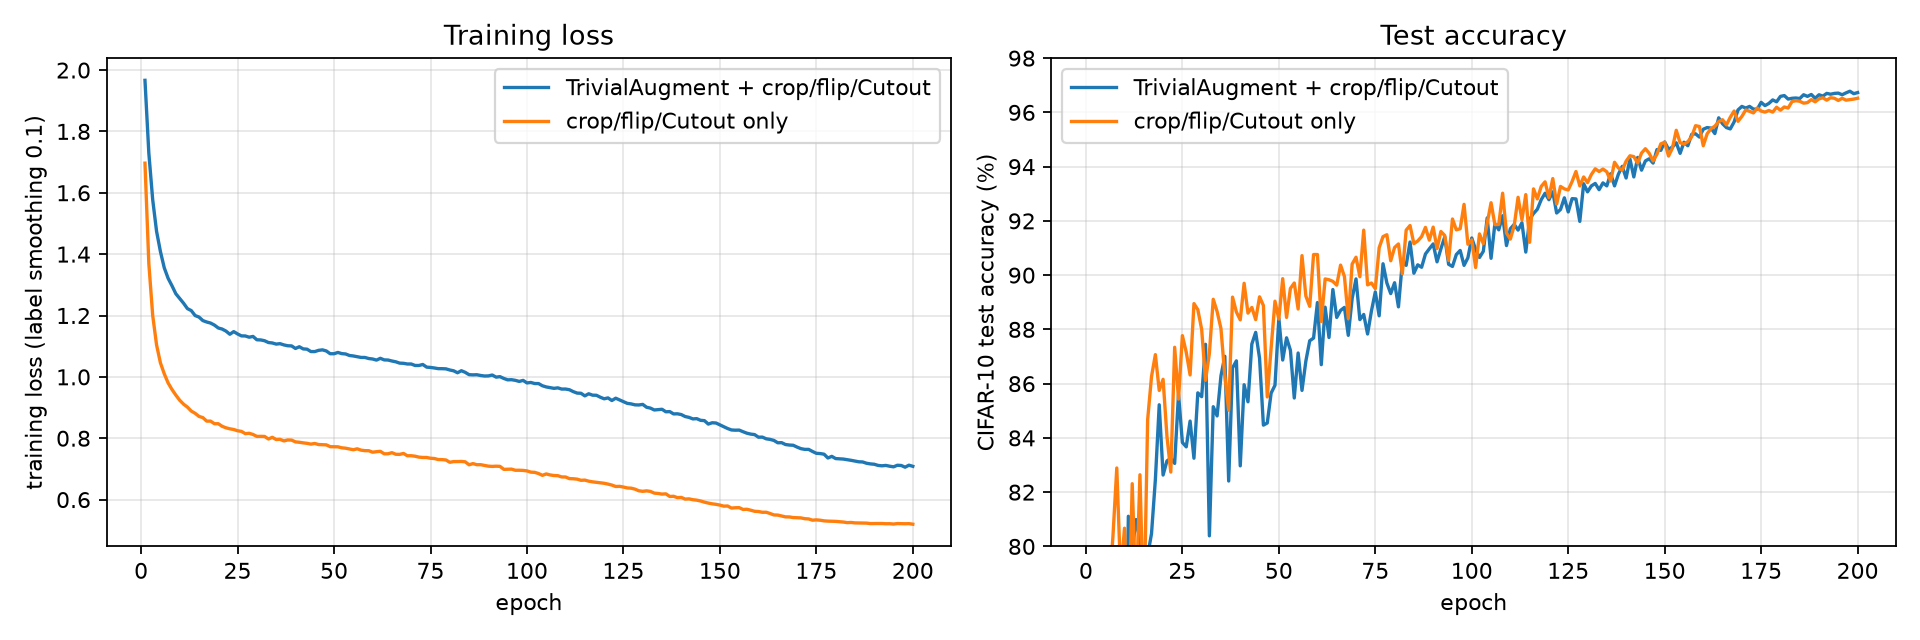
\includegraphics[width=0.85\textwidth]{../figures/curves.png}
\caption{200-epoch training with and without TrivialAugment. Left: training loss (with label smoothing). Right:
CIFAR-10 test accuracy after each epoch (no TTA).}
\label{fig:curves}
\end{figure*}

\subsection{Knowledge Distillation}
The parameter limit applies to the submitted model only, and the project allows teacher-student distillation, so I
trained larger teachers and distilled them into layout B \cite{hinton2015distilling}. For a batch of augmented
images $x$, the student $s$ minimizes
\begin{equation*}
\mathcal{L} = \alpha\,\mathrm{CE}(y, s(x)) + (1-\alpha)\,T^2\,\mathrm{KL}\big(\bar p_T(x)\,\|\,\sigma(s(x)/T)\big),
\end{equation*}
where $\bar p_T(x)$ is the average of the teachers' softmax outputs at temperature $T$ and $\sigma$ is the softmax.
Following \citet{beyer2022knowledge}, the teachers see exactly the same augmented image as the student
(``consistent'' teaching), so the target changes with every crop, Cutout and TrivialAugment operation, and the
student is trained for a long time (``patient'' teaching). I used $\alpha=0.1$ and $T=1$, because my teachers were
trained with label smoothing, and \citet{chandrasegaran2022revisiting} found such teachers distill well at low
temperature but poorly at high temperature. The student uses the same recipe as before (TrivialAugment, label
smoothing on the hard-label term).

\begin{table}[t]
\centering
\small
\setlength{\tabcolsep}{4pt}
\begin{tabular}{lcccc}
\toprule
Teachers (runs) & Params & Ep. & Test & + TTA \\
\midrule
B (4) & 4.78M & 200 & 96.5 to 96.8 & 96.8 to 97.1 \\
Wide (2) & 11.09M & 300 & 97.41, 97.45 & 97.61, 97.66 \\
Big (2) & 36.69M & 300 & 97.66, 97.67 & 97.86, 97.92 \\
Big + CutMix (2) & 36.69M & 400 & 97.66, 97.85 & 97.83, 97.99 \\
\bottomrule
\end{tabular}
\caption{Teachers, used only during training and never submitted. Wide: channels 128-256-512, two blocks per layer.
Big: channels 160-320-640, four blocks per layer.}
\label{tab:teachers}
\end{table}

\begin{table}[t]
\centering
\small
\setlength{\tabcolsep}{3pt}
\setlength{\tabcolsep}{2.5pt}
\begin{tabular}{lccccccc}
\toprule
Run & Teachers & CM & Ep. & Test & TTA & Pub. & Priv. \\
\midrule
plain & none & 0 & 200 & 96.73 & 97.00 & .884 & .852 \\
kd & 4B & 0 & 300 & 97.10 & 97.27 & .885 & .863 \\
kd2 & 2W+2B & 0 & 500 & 97.51 & 97.58 & & \\
kd3 & 2W+2B & 0 & 800 & 97.57 & 97.69 & .887 & .867 \\
kd4 & 2L+2W & 0 & 800 & 97.52 & 97.68 & & \\
kd5 & 2L+2W & 0.5 & 800 & 97.61 & 97.73 & .895 & .867 \\
kd7 & 2L+2W & 0.5 & 1200 & 97.76 & 97.86 & .890 & .872 \\
kd6 & 2L+2W & 1 & 1200 & 97.69 & 97.77 & .903 & .871 \\
kd8 & 2C+2W & 1 & 1200 & 97.67 & 97.72 & .907 & .874 \\
\textbf{kd10} & \textbf{2C+2W} & \textbf{1} & \textbf{1200} & \textbf{97.82} & \textbf{97.89} & \textbf{.907} & \textbf{.871} \\
\bottomrule
\end{tabular}
\caption{All students use layout B (4.78M parameters). Teachers: B, W(ide), L (big), C (big + CutMix). CM: probability
of CutMix per batch. Test and TTA: CIFAR-10 accuracy in \%. Pub.\ and Priv.: Kaggle score on the public and the hidden
half, blank if not uploaded. kd8 and kd10 differ only in seed.}
\label{tab:kd}
\end{table}

Tables~\ref{tab:teachers} and \ref{tab:kd} and Figure~\ref{fig:kd} show the result. With four B-sized teachers the
student reached 97.27\% (TTA), close to the 97.31\% of the ensemble of those teachers. Replacing two of them with wider
networks raised the student to 97.58\% after 500 epochs and 97.69\% after 800. Figure~\ref{fig:kd} plots accuracy
against the fraction of the schedule: the distilled runs are ahead of plain training throughout.

\begin{figure}[t]
\centering
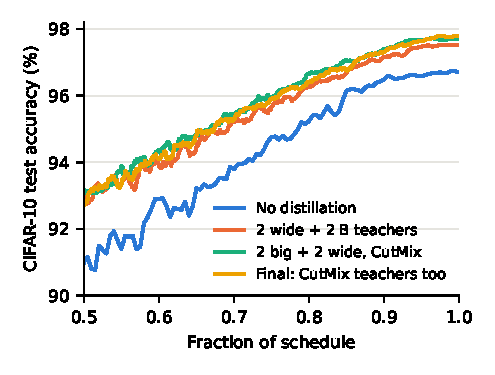
\includegraphics[width=\columnwidth]{../figures/kd_curves.pdf}
\caption{CIFAR-10 test accuracy (no TTA) over the second half of training, against the fraction of each run's schedule,
averaged over 1\% of the schedule.}
\label{fig:kd}
\end{figure}

\subsection{Bigger Teachers and CutMix}
Better teachers alone stopped helping. Big teachers reach about 97.9\% (TTA), but the student kd4 stayed at 97.68\%,
the same as kd3. I then added CutMix \cite{yun2019cutmix}: with probability CM, a random rectangle of each image is
replaced by the same rectangle from another image in the batch. The hard-label loss is weighted by the area of each
image, and the teachers see the mixed image, so the distillation target is simply what they predict for it.

On CIFAR-10 this gave small gains that are close to the difference between seeds. On the competition images it did
more: the public score was 0.887 without it (kd3), 0.895 at CM $=0.5$ with the bigger teachers (kd5), and 0.903 at
CM $=1$ (kd6). Training the big teachers with CutMix as well raised it to 0.907 (kd8 and kd10). Since each public score
has noise (see below), I read this as a trend and not as an exact ranking of the runs. On the hidden half, shown after
the competition, the same steps gave a smaller gain (0.867, 0.867, 0.871, 0.874).

\subsection{Compute}
The pilots, the 50- and 200-epoch runs, and the first distillation round ran on one RTX 4090 Laptop GPU (32 minutes
for 200 epochs). All later runs used A100 GPUs on NYU HPC (Cloud Bursting): about 30 minutes for a wide teacher, 73 to
98 minutes for a big teacher, and about 5 hours for a 1200-epoch student. A further student (four big teachers) was
cancelled by the cluster at epochs 973 and 1000 of 1200, so it has no result. On HPC the standard CIFAR-10 download was
blocked, so I used the copy on Hugging Face (\texttt{uoft-cs/cifar10}); I verified that its test set is byte-identical
and that its training set has the same 50,000 images and labels (in a different order, which does not matter here).

\section{Results}

\subsection{Final Model}
The final model is layout B distilled for 1200 epochs from two CutMix-trained big teachers and two wide teachers, with
CutMix on every batch (\texttt{kd10\_B\_e1200\_cmT\_s3}). In the project's notation: $N=3$,
$B=(2,2,2)$, $C=(84,168,336)$, $F=(3,3,3)$, $K=(1,1,1)$ where the shape changes, and $P=8$ (Figure~\ref{fig:arch},
Table~\ref{tab:params}).

\begin{figure*}[t]
\centering
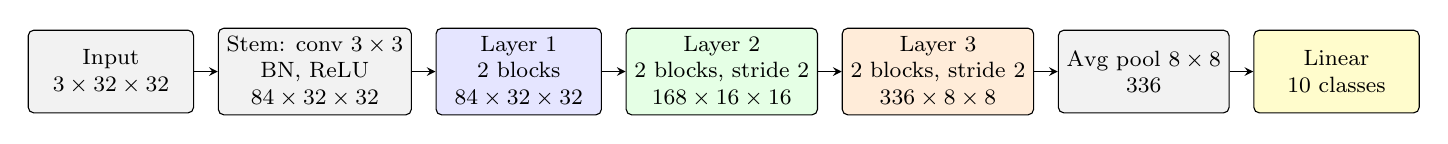
\begin{tikzpicture}[font=\footnotesize, box/.style={draw, rounded corners=2pt, align=center, minimum height=1.05cm, minimum width=2.1cm, inner sep=3pt}, >=stealth, node distance=0.3cm]
\node[box, fill=gray!10] (in) {Input\\$3\times32\times32$};
\node[box, fill=gray!10, right=of in] (stem) {Stem: conv $3\times3$\\BN, ReLU\\$84\times32\times32$};
\node[box, fill=blue!10, right=of stem] (l1) {Layer 1\\2 blocks\\$84\times32\times32$};
\node[box, fill=green!10, right=of l1] (l2) {Layer 2\\2 blocks, stride 2\\$168\times16\times16$};
\node[box, fill=orange!15, right=of l2] (l3) {Layer 3\\2 blocks, stride 2\\$336\times8\times8$};
\node[box, fill=gray!10, right=of l3] (pool) {Avg pool $8\times8$\\336};
\node[box, fill=yellow!20, right=of pool] (fc) {Linear\\10 classes};
\foreach \a/\b in {in/stem, stem/l1, l1/l2, l2/l3, l3/pool, pool/fc} \draw[->] (\a) -- (\b);
\end{tikzpicture}

\vspace{0.3cm}
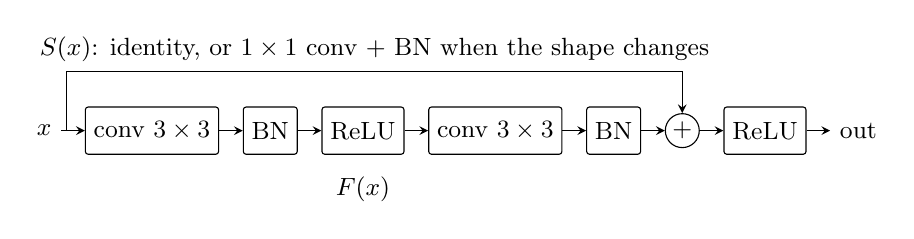
\begin{tikzpicture}[font=\small, b/.style={draw, rounded corners=1pt, minimum height=0.6cm, inner sep=3pt}, >=stealth, node distance=0.3cm]
\node (x) {$x$};
\node[b, right=of x] (c1) {conv $3\times3$};
\node[b, right=of c1] (n1) {BN};
\node[b, right=of n1] (r1) {ReLU};
\node[b, right=of r1] (c2) {conv $3\times3$};
\node[b, right=of c2] (n2) {BN};
\node[draw, circle, inner sep=1pt, right=of n2] (p) {$+$};
\node[b, right=of p] (r2) {ReLU};
\node[right=of r2] (o) {out};
\foreach \a/\b in {x/c1, c1/n1, n1/r1, r1/c2, c2/n2, n2/p, p/r2, r2/o} \draw[->] (\a) -- (\b);
\draw[->] ([xshift=2pt]x.east) |- ++(0,0.75) -| node[pos=0.25, above] {$S(x)$: identity, or $1\times1$ conv + BN when the shape changes} (p.north);
\node[below=0.15cm of r1] {$F(x)$};
\end{tikzpicture}
\caption{Final architecture (top) and the basic block (bottom). The first block of layers 2 and 3 uses stride 2 and a
$1\times1$ projection on the skip path; all other skips are the identity.}
\label{fig:arch}
\end{figure*}

\begin{table}[t]
\centering
\small
\begin{tabular}{lccr}
\toprule
Part & Output & Details & Params \\
\midrule
Stem & $84\times32^2$ & conv $3\times3$, BN & 2,436 \\
Layer 1 & $84\times32^2$ & 2 blocks & 254,688 \\
Layer 2 & $168\times16^2$ & 2 blocks & 904,848 \\
Layer 3 & $336\times8^2$ & 2 blocks & 3,616,032 \\
Head & 10 & pool, linear & 3,370 \\
\midrule
\textbf{Total} & & & \textbf{4,781,374} \\
\bottomrule
\end{tabular}
\caption{Trainable parameters of the final model (checked with \texttt{torchsummary}; limit 5,000,000). Layer 3
holds 75.6\% of them.}
\label{tab:params}
\end{table}

\subsection{CIFAR-10 Test Accuracy}
The final model reaches \textbf{97.82\%} on the 10,000 CIFAR-10 test images and \textbf{97.89\%} with flip TTA
(Table~\ref{tab:class}). Most errors are between cats and dogs (37 cats predicted as dogs and 30 dogs as cats, down
from 51 and 34 without distillation), followed by trucks predicted as cars (11) and airplanes predicted as ships (10,
down from 19).

\begin{table}[t]
\centering
\small
\setlength{\tabcolsep}{3pt}
\begin{tabular}{ccccccccccc}
\toprule
plane & car & bird & cat & deer & dog & frog & horse & ship & truck \\
\midrule
98.4 & 99.0 & 97.5 & 94.7 & 98.6 & 96.2 & 99.2 & 98.5 & 98.9 & 98.1 \\
\bottomrule
\end{tabular}
\caption{Per-class test accuracy (\%) of the final model with flip TTA, averaging softmax outputs as the Kaggle predictions do (97.9\% overall).}
\label{tab:class}
\end{table}

\subsection{Competition Test Set}
The competition's 2,000 test images are a re-collected, CIFAR-like set rather than the standard test set: they look
like natural CIFAR images (no added noise or compression), but they are slightly brighter (mean pixel 125.1 against
121.5) and the model is less confident on them (mean top-class probability 0.78 against 0.83). Such re-collected test
sets are known to lower accuracy by several points \cite{recht2019imagenet}. The public score uses half of the images
(about 1,000), so it has a standard error of roughly 1 point; each image is worth 0.001. Table~\ref{tab:kd} lists the
main submissions, and Kaggle lets me pick two for the final ranking: kd10 and kd8. The final score is the better of
the two on the hidden half: 0.874 (kd8), rank 28 of 81 teams.

CIFAR-10 accuracy was a weak guide to this score. kd7 beat kd6 on CIFAR-10 (97.86\% against 97.77\%) but scored 1.3
points lower, and kd8 and kd10 tie at 0.907 while differing on 92 of the 2,000 predictions. The final model changes
7.0\% of the competition predictions compared with the plain model, against 2.1\% of the CIFAR-10 predictions, so the
two test sets behave differently.

The hidden half was harder than the public half (0.86 to 0.88 against 0.88 to 0.91), and it reordered close
submissions: the class-balanced predictions, worst on the public half among my late uploads, were best on the hidden
half (0.879), and the shifted kd8 beat plain kd8 there. Differences of a few images on either half are noise. Over the
whole project, distillation still raised the hidden-half score from 0.852 to 0.871 to 0.874.

\begin{table}[t]
\centering
\small
\setlength{\tabcolsep}{4pt}
\begin{tabular}{lccc}
\toprule
Prediction & CIFAR-10 & Public & Private \\
\midrule
\textbf{kd10, flip TTA (final)} & \textbf{97.91} & \textbf{0.907} & \textbf{0.871} \\
kd10 + 5 shifts & 97.94 & 0.903 & 0.873 \\
kd10 + 9 shifts & 97.95 & 0.902 & 0.867 \\
kd8, flip TTA (other pick) & 97.71 & 0.907 & 0.874 \\
kd8 + 9 shifts & 97.82 & 0.902 & 0.878 \\
kd10 + class balancing & see text & 0.895 & 0.879 \\
\bottomrule
\end{tabular}
\caption{Test-time ideas I tried and did not use. Shifts: also averaging 1-pixel shifts of the image. CIFAR-10 accuracy
here averages softmax outputs, as the Kaggle predictions do. Private: the hidden half, shown only after the competition
closed. Final leaderboard: rank 28 of 81 teams, 0.874 (kd8, the better of my two picks on the hidden half).}
\label{tab:kaggle}
\end{table}

\subsection{Test-Time Ideas I Rejected}
The professor allowed test-time BN adaptation \cite{schneider2020improving} and class-balanced prediction on the course
Slack, provided they are disclosed. I tested both, using the unlabeled test images but no retraining, and the final
predictions use neither (\texttt{test\_time\_checks.py}).
\begin{itemize}
\item \textbf{BN statistics from the test images.} On random 2,000-image CIFAR-10 test subsets, replacing the BN
statistics with those of the subset lowered accuracy from 97.89\% to 96.32\%, probably because the training statistics
come from heavily augmented images. Mixing 20\% of them into the training statistics gave 97.88\%. I did not upload this.
\item \textbf{Class balancing.} I shifted the class scores until each class was predicted about equally often. On
CIFAR-10 subsets this gave 98.21\% against 98.02\% when the subset had equal classes, but 96.20\% against 97.90\% on
random subsets. On Kaggle it changed 66 predictions and scored 0.895, which is 12 images worse on the public half.
\item \textbf{Shift averaging} (Table~\ref{tab:kaggle}). It gained up to 0.11 points on CIFAR-10 but lost 4 or 5 images
on the public half, on each model I uploaded. On the hidden half the results were mixed (Table~\ref{tab:kaggle}), so I
cannot call either idea better or worse than plain flip TTA.
\end{itemize}

\section{Lessons Learned}
\begin{itemize}
\item \textbf{Spend the budget on width where the resolution is high.} A fourth layer at $4\times4$ was a poor use
of parameters compared with wider early layers.
\item \textbf{The recipe matters more than the layout.} The same network went from 92.4\% (15 epochs) to 97.8\%
(long training and distillation), while the four layouts were within 2.4 points of each other.
\item \textbf{Judge augmentation at the final training length.} From the 50-epoch runs alone I would have dropped
TrivialAugment, which was the better choice at 200 epochs.
\item \textbf{Distillation is a free lunch at inference time, up to a point.} Teachers can be as large as the training
budget allows, since only the student is submitted. Going from 11M to 37M teachers no longer helped by itself; CutMix
and longer schedules did.
\item \textbf{CIFAR-10 is a weak guide on a shifted test set.} Regularization that changed little on CIFAR-10 moved the
competition score the most, and test-time ideas that looked safe on CIFAR-10 lowered the public score.
\item \textbf{Half a test set is a noisy judge.} With about 1,000 images per half, choices made on the public score
did not all hold on the hidden half; only large, consistent gains (here, distillation) did.
\item \textbf{A fast pipeline pays off.} Two-minute pilots made it cheap to test ideas before long runs.
\item \textbf{Limitations.} I used the CIFAR-10 test set to compare the final candidates, so those numbers may be
slightly optimistic. I also chose among 12 uploads using the public score, and the hidden half confirmed that 0.907
was optimistic: my final entry scored 0.874 there. Two seeds of the same recipe gave 97.72\% and 97.89\%, so smaller
gaps on CIFAR-10 mean little. I did not tune the distillation settings ($\alpha$, $T$).
\end{itemize}

\bibliography{refs}

\end{document}
